\documentclass[12pt,a4paper]{ctexart}
\usepackage[left=2.5cm,right=2.5cm,top=2.5cm,bottom=2.5cm]{geometry}
\usepackage{tikz}
\usepackage{tabularx}
\usepackage{booktabs}
\usepackage{enumitem}
\usepackage{xcolor}
\usepackage{hyperref}
\usepackage{fancyhdr}
\usepackage{amsmath}
\usepackage{graphicx}
\usepackage{caption}
\usepackage{float}
\usepackage{multirow}

\setlength{\parskip}{6pt}
\setlength{\parindent}{0pt}
\setlength{\headheight}{14.5pt}
\pagestyle{fancy}
\fancyhf{}
\fancyhead[L]{\textbf{求解结果文档}}
\fancyhead[R]{\thepage}
\renewcommand{\headrulewidth}{1pt}

\newcolumntype{C}{>{\centering\arraybackslash}X}
\newcolumntype{L}{>{\raggedright\arraybackslash}X}

\definecolor{headblue}{RGB}{26,60,110}
\definecolor{accentblue}{RGB}{43,92,158}

\title{\vspace{-2cm}\textbf{\Huge 求解结果文档}\\[6pt]
\large 2026 高教社杯全国大学生数学建模竞赛 B 题\\[2pt]
\large 无线电干扰源的快速自动定位与清除}
\author{}
\date{}

\begin{document}

\maketitle
\vspace{-1.5cm}

% ============================================================
\section{问题一结果汇总}
% ============================================================

本问解决了"给定若干检测点坐标及其示向度，如何计算交会定位区域直径，并判断以该直径为直径的圆能否覆盖该区域"这一问题，产出了一套可直接调用的凸多边形求解算法与一个充要的覆盖判据。示向度误差按 $[-1^\circ,1^\circ]$ 处理，定位区域被表达为 $2m$ 个楔形半平面与目标圆域的交，用 Sutherland--Hodgman 逐次裁剪求顶点，再用旋转卡壳求直径。

表 \ref{tab:r1-key} 给出关键数值结果。算法层面，旋转卡壳法与顶点对暴力枚举法在全部算例上的直径偏差不超过 $10^{-9}$ 米，互为校验；判据层面，覆盖结论由 Thales 逆定理给出，可改写为两个符号量 $\sigma_B=(B-A)\cdot(B-C)$ 与 $\sigma_D=(D-A)\cdot(D-C)$ 均非正。

\begin{table}[H]
  \centering
  \caption{问题一关键结果}
  \label{tab:r1-key}
  \begin{tabularx}{\textwidth}{LC}
    \toprule
    指标 & 数值 \\
    \midrule
    示范构型定位区域直径 $D_P$ & $56.7078$ m \\
    示范构型最小包围圆半径 / 直径 & $0.500000$（直径圆恰好外接） \\
    蒙特卡洛构型总数 / 有效构型数 & $5000$ / $4860$ \\
    非空构型占比 & $100.00\%$ \\
    无界退化构型占比（未加圆域约束） & $2.80\%$ \\
    \textbf{直径圆覆盖率（纯交会四边形）} & $\mathbf{98.99\%}$ \\
    直径圆覆盖率（叠加目标圆域截断） & $96.28\%$ \\
    定位区域直径 均值 / 中位数 / 标准差 & $402.53$ / $157.96$ / $959.38$ m \\
    直径最大值 / 最小值 & $19149.05$ / $10.04$ m \\
    最小包围圆半径与直径之比 均值 / 最大值 & $0.500001$ / $0.500280$（Jung 上界 $0.577350$） \\
    覆盖失败构型超出量 均值 / 最大值 & $0.4928$ / $1.1697$ m \\
    失败构型超出量占直径比例 最大 & $1.37\%$ \\
    \bottomrule
  \end{tabularx}
\end{table}

从表 \ref{tab:r1-key} 可以看出三点结论。第一，直径圆不能保证覆盖定位区域，其成立的充要条件是 $\angle ABC\ge90^\circ$ 且 $\angle ADC\ge90^\circ$（$AC$ 为直径）；第二，覆盖失败的频率很低（约 $1\%$），且失败仅发生在两视线交会角接近 $90^\circ$ 的临界构型上，此时定位区域趋近矩形而矩形恰是 Thales 判据的临界形状；第三，失败的绝对幅度极小，超出量最大仅 $1.17$ 米、平均不足半米，相对于清除半径 $20$ 米的要求完全可以忽略。

\begin{figure}[H]
  \centering
  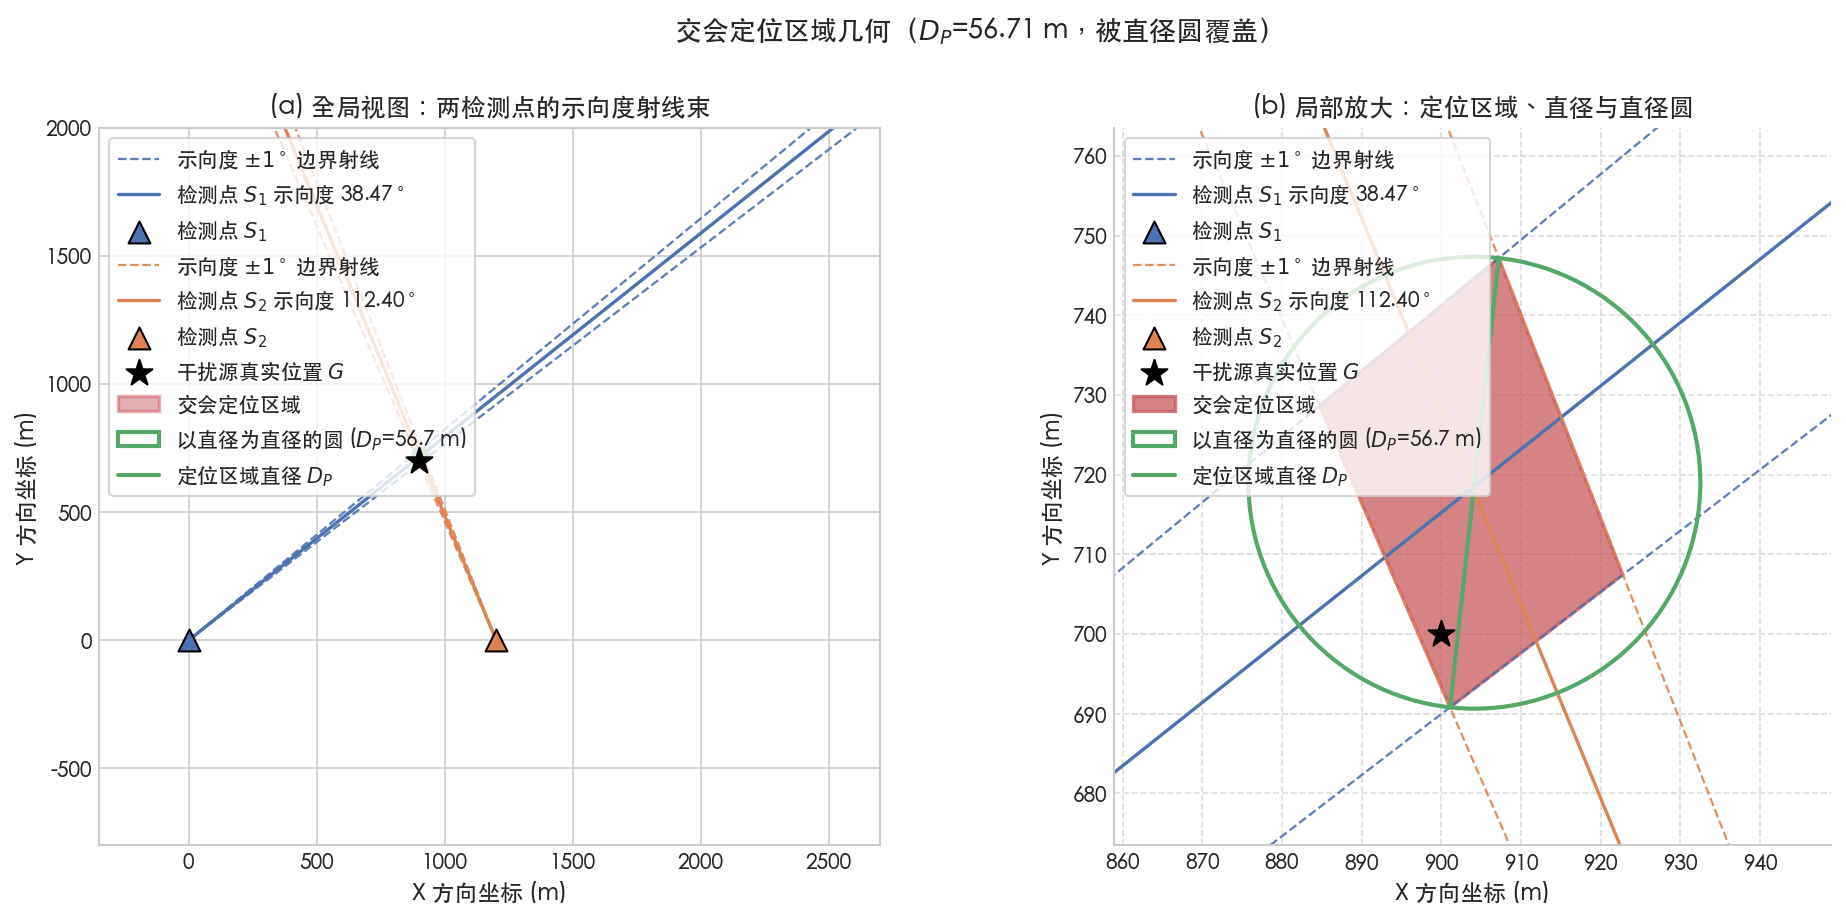
\includegraphics[width=0.8\textwidth]{问题一/figures/交会定位区域示意图.png}
  \caption{交会定位区域、直径与直径圆}
  \label{fig:r1-1}
\end{figure}

如图 \ref{fig:r1-1} 所示，两条示向度射线束在目标附近相夹形成狭长的凸四边形，其长对角线的中点恰为直径圆圆心，四个顶点几乎全部落在圆上。

\begin{figure}[H]
  \centering
  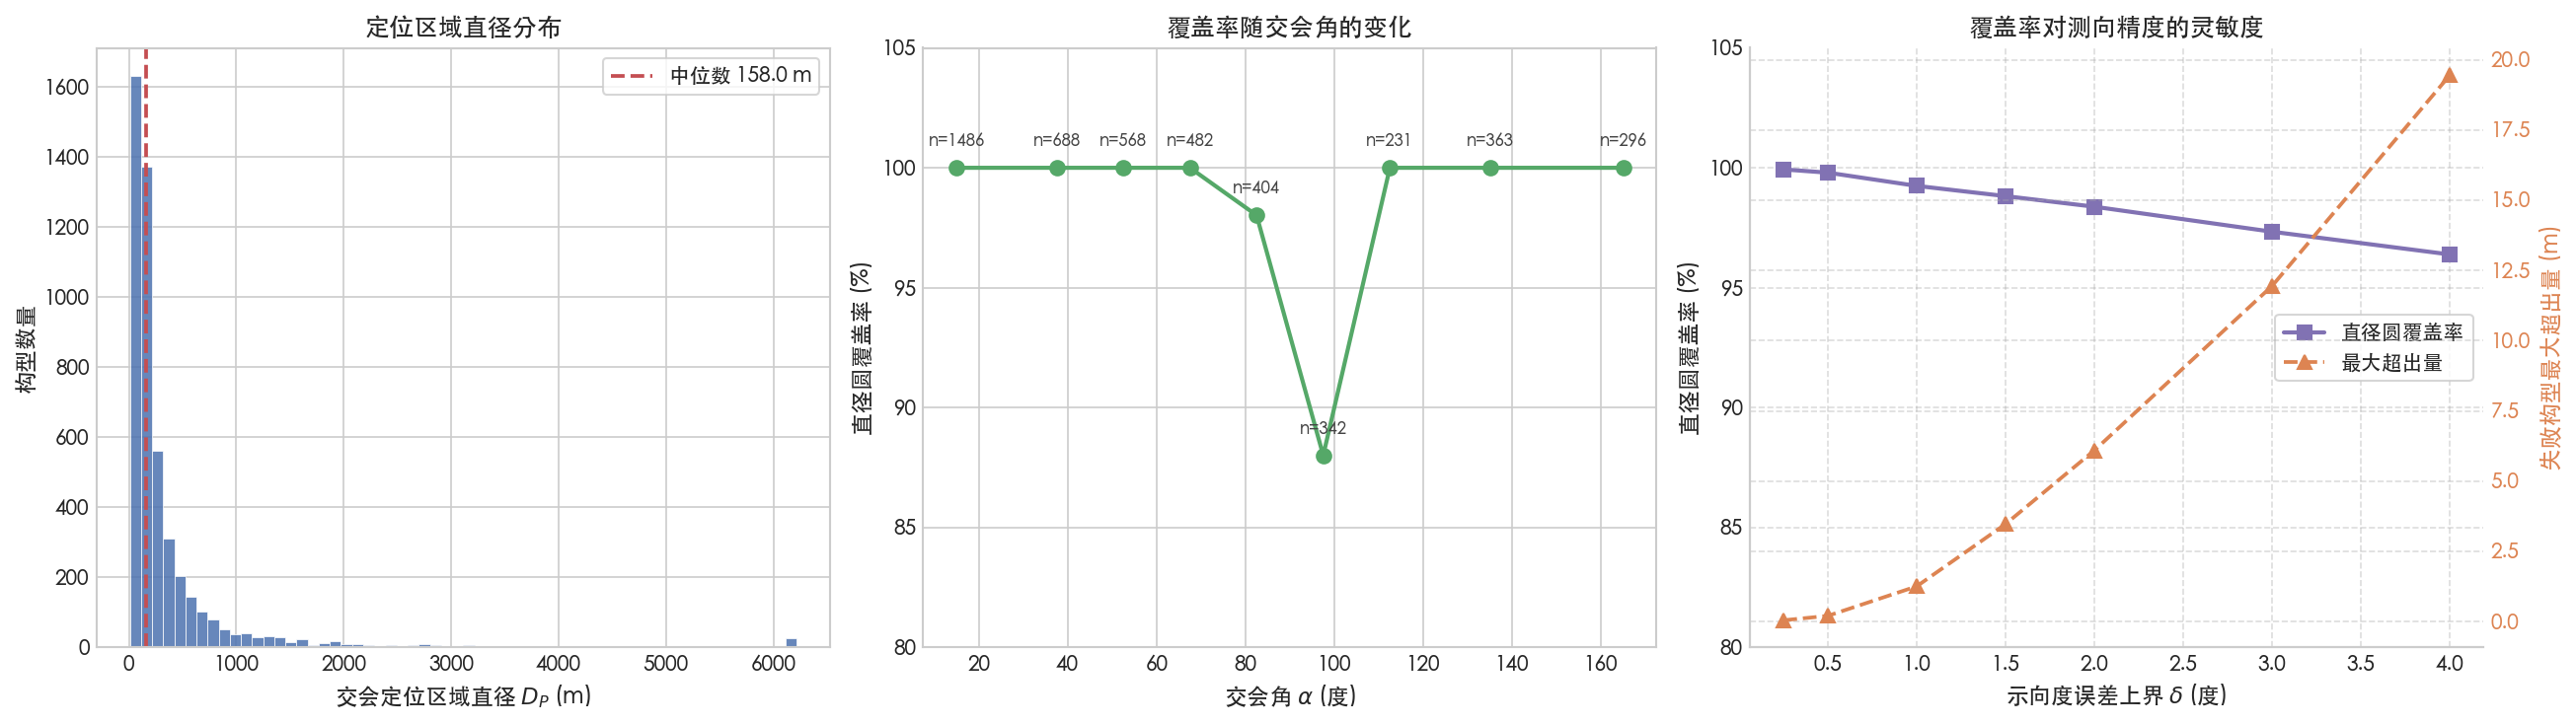
\includegraphics[width=0.8\textwidth]{问题一/figures/直径圆覆盖率与直径分布图.png}
  \caption{定位区域直径分布、覆盖率随交会角的变化与测向精度灵敏度}
  \label{fig:r1-2}
\end{figure}

图 \ref{fig:r1-2} 显示直径分布呈显著右偏（中位数 $158$ 米、均值 $403$ 米），覆盖率在交会角 $90^\circ$ 附近出现明显凹陷（$(90^\circ,105^\circ]$ 区间降至 $88.01\%$），而测向精度由 $1^\circ$ 收紧至 $0.25^\circ$ 时覆盖率升至 $99.93\%$。

% ============================================================
\section{问题二结果汇总}
% ============================================================

本问解决了"已知某全向干扰源在一个检测点处的示向度，第二个检测点应选在哪里"这一问题，给出了完整的解析最优结论、两种稳健准则下的数值最优布站以及一片可执行的候选区域。

设第一检测点位于原点、示向度方向为 $+x$ 轴，基线长度为 $b$、基线方位角与视线夹角为 $\varphi$。在垂直布站（$\varphi=90^\circ$）这一特例下，定位误差为 $E(b;r)=\frac{\delta}{b}\sqrt{(r^2+b^2)(4r^2+b^2)}$，令 $t=b^2/r^2$ 则 $E\propto\sqrt{t+5+4/t}$，在 $t=2$ 处取极小，由此得到闭式结论
\begin{equation}
b^{*}=\sqrt2\,r,\qquad \alpha^{*}=\arccos\frac{1}{\sqrt3}=54.74^\circ,\qquad E_{\min}=3\delta r=0.052360\,r .
\end{equation}
表 \ref{tab:r2-key} 给出一般布站下的数值最优结果。

\begin{table}[H]
  \centering
  \caption{问题二关键结果}
  \label{tab:r2-key}
  \begin{tabularx}{\textwidth}{LCCC}
    \toprule
    准则 & 最优基线 $b^*$ (m) & 最优方位角 $\varphi^*$ & 期望定位误差 (m) \\
    \midrule
    期望准则（主） & $1401.4$ & $20.03^\circ$ & $\mathbf{22.19}$ \\
    极小化极大准则 & $1499.3$ & $41.09^\circ$ & $26.90$（最坏误差 $39.92$） \\
    限定垂直布站（次优） & $1510.0$ & $90.00^\circ$ & $55.73$ \\
    \midrule
    \multicolumn{4}{l}{\textbf{候选区域}（$5\%$ 精度容差）：$b\in[1230,1630]$ m，$\varphi\in[14^\circ,29^\circ]$（含镜像）} \\
    \bottomrule
  \end{tabularx}
\end{table}

表 \ref{tab:r2-key} 的核心发现是：在计入全可行域不确定性后，最优布站并非教科书中常引用的垂直布站，而是取方位角约 $20^\circ$、基线约 $1401$ 米，此时期望定位误差 $22.19$ 米；垂直布站即使把基线放长到 $1510$ 米，期望误差仍为 $55.73$ 米，是最优方案的 $2.5$ 倍。若采用极小化极大准则，最优解向垂直方向移动至 $41.09^\circ$，期望误差略增至 $26.90$ 米，但最坏误差由 $72.87$ 米压缩至 $39.92$ 米。

\begin{figure}[H]
  \centering
  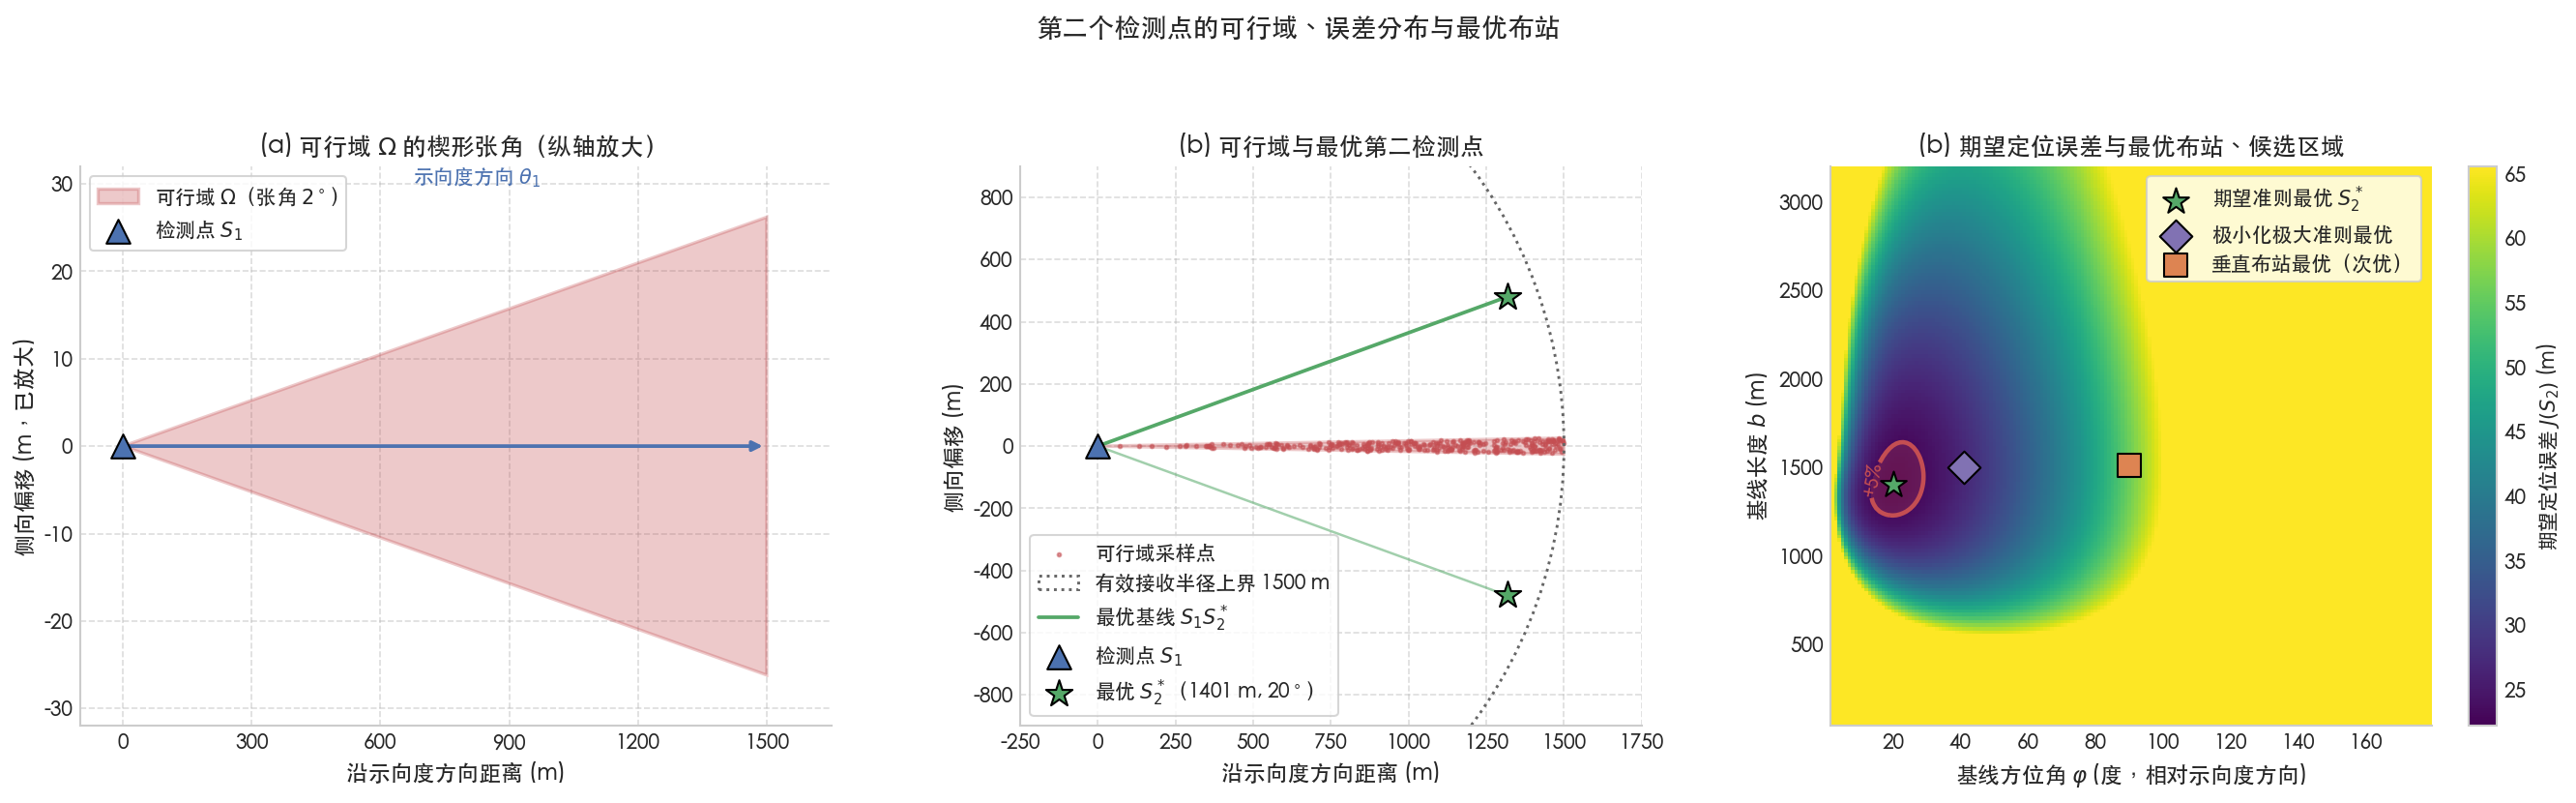
\includegraphics[width=0.8\textwidth]{问题二/figures/可行域与候选区域示意图.png}
  \caption{干扰源可行域、定位误差分布与最优第二检测点}
  \label{fig:r2-1}
\end{figure}

图 \ref{fig:r2-1}(a) 显示单次示向度给出的可行域张角仅 $2^\circ$，在 $1500$ 米处侧向宽度仅约 $52$ 米，这正是径向不确定度巨大的几何根源。

\begin{figure}[H]
  \centering
  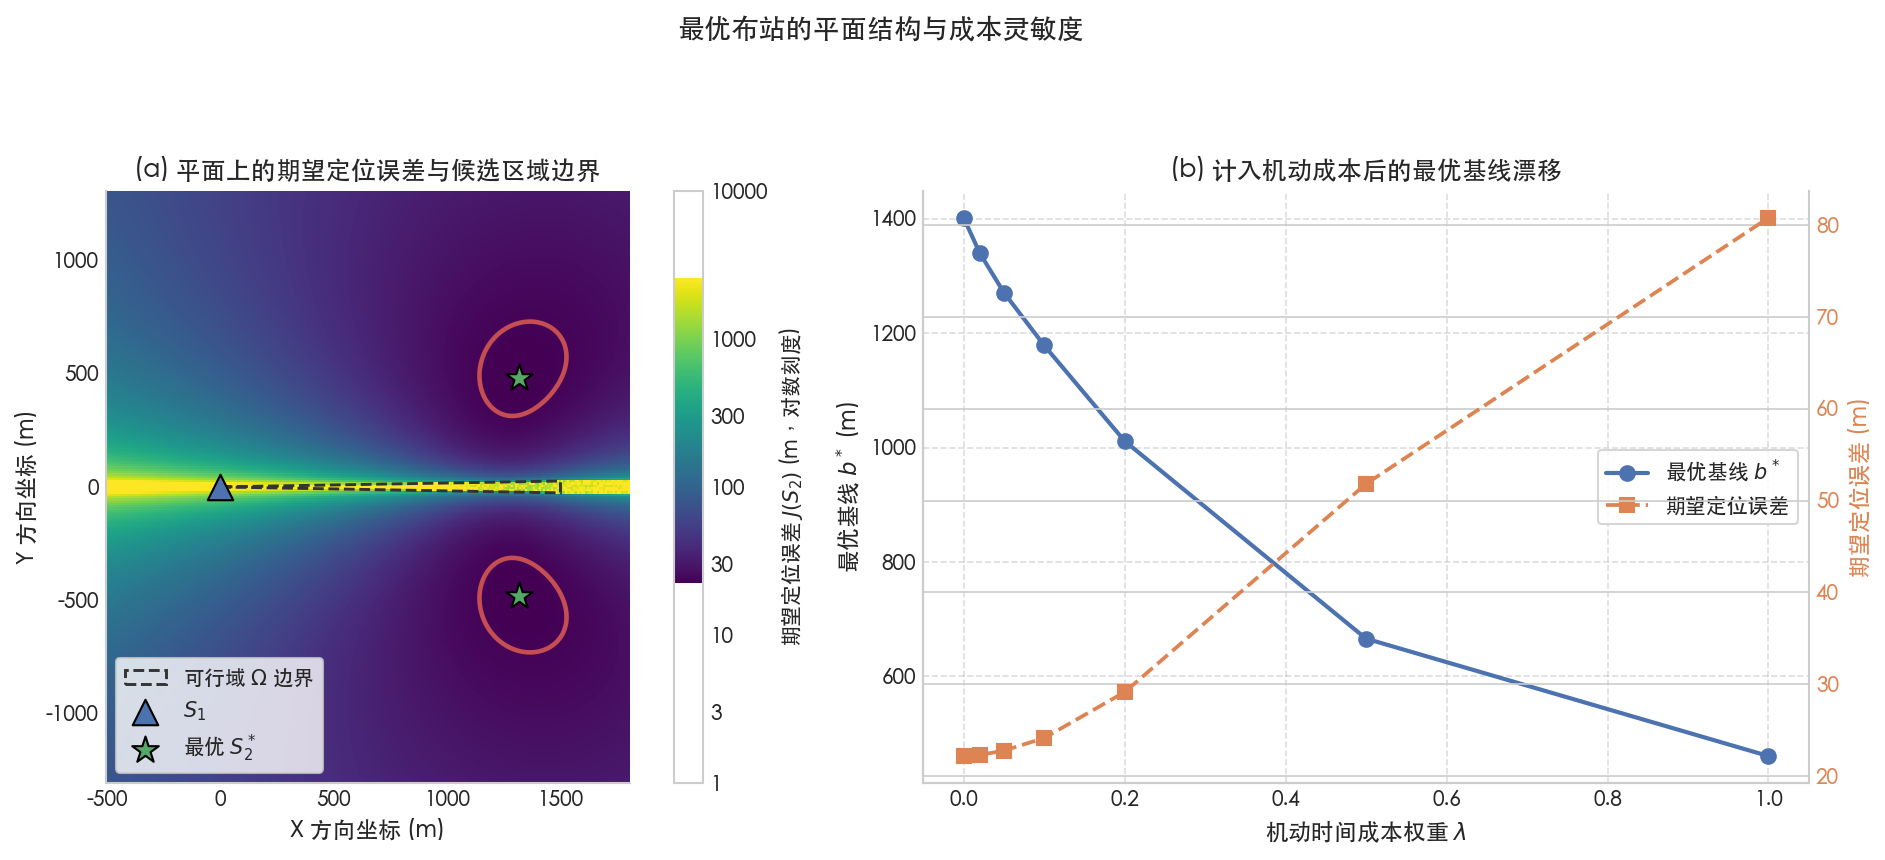
\includegraphics[width=0.8\textwidth]{问题二/figures/最优布站平面结构与成本灵敏度图.png}
  \caption{平面上期望定位误差的结构与机动成本灵敏度}
  \label{fig:r2-2}
\end{figure}

图 \ref{fig:r2-2}(a) 显示目标函数沿视线方向存在一条高误差脊线（共线观测导致 $\sin\alpha\to0$），最优第二检测点落于脊线两侧对称的低误差盆地中。图 \ref{fig:r2-2}(b) 给出计入机动成本后的漂移：成本权重 $\lambda$ 由 $0$ 增至 $1.0$ 时，最优基线由 $1401$ 米收缩至 $461$ 米，方位角向 $56.3^\circ$ 靠拢，趋近解析最优交会角 $54.74^\circ$。

% ============================================================
\section{问题三结果汇总}
% ============================================================

本问解决了"如何在 $20$ 分钟程序运行时限内、以最短虚拟时间清除全部 $10\sim16$ 个位置与频道均未知的全向干扰源"这一问题，产出了一套"全域粗探—交会定距—迭代逼近—就地清除"的四阶段策略，并给出了时间模型与理论下界。

策略的第一个支柱是保证覆盖网。由 Kershner 定理，$6$ 个半径 $1000$ 米的圆盘最多覆盖半径 $1732.05$ 米的圆域，小于目标区域半径 $1800$ 米，故观测点数下界为 $7$。取"$1$ 中心 $+ 6$ 环点"构型，求解得最优环半径 $d^{*}=1558.85$ 米（最小覆盖半径 $900.00$ 米）；令覆盖半径恰为 $1000$ 米得两个根 $d_1=1122.96$ 米与 $d_2=1733.50$ 米，取最小根 $d_1$ 使巡回周长最短（$6737.7$ 米）。

策略的第二个支柱是定位精度阈值。由问题二结论 $E=3\delta r$ 与清除半径 $20$ 米反解，得必须逼近到 $r\le381.97$ 米以内。

\begin{table}[H]
  \centering
  \caption{问题三虚拟时间模型与理论下界（侧移系数 $\beta_l=0.25$）}
  \label{tab:r3-time}
  \begin{tabular}{cccccc}
    \toprule
    干扰源个数 $N$ & 粗探时间 (s) & 清除移动 (s) & 清除动作 (s) & 总时间 (s) & 平均定位清除时间 (s) \\
    \midrule
    $10$ & $2180.5$ & $1796.8$ & $170.0$ & $4147.4$ & $414.7$ \\
    $11$ & $2180.5$ & $1884.6$ & $187.0$ & $4252.1$ & $386.6$ \\
    $12$ & $2180.5$ & $1968.3$ & $204.0$ & $4352.9$ & $362.7$ \\
    $13$ & $2180.5$ & $2048.7$ & $221.0$ & $4450.3$ & $342.3$ \\
    $14$ & $2180.5$ & $2126.1$ & $238.0$ & $4544.6$ & $324.6$ \\
    $15$ & $2180.5$ & $2200.7$ & $255.0$ & $4636.2$ & $309.1$ \\
    $16$ & $2180.5$ & $2272.9$ & $272.0$ & $4725.4$ & $295.3$ \\
    \midrule
    \multicolumn{6}{l}{理想下界 $T_{\mathrm{lb}}=L_{\mathrm{TSP}}/v+16N$：$N=13$ 时为 $1847.0$ s} \\
    \bottomrule
  \end{tabular}
\end{table}

由表 \ref{tab:r3-time} 可见，粗探阶段固定耗时 $2180.5$ 秒，由 $6737.7$ 米巡回位移（$1347.5$ 秒）、$140$ 次检测（$700$ 秒）与 $133$ 次频道切换（$133$ 秒）构成，约占模型总时间的一半。总时间随 $N$ 由 $4147$ 秒增至 $4725$ 秒，而平均定位清除时间由 $414.7$ 秒降至 $295.3$ 秒——目标越多，粗探成本被分摊得越充分，单位清除成本反而越低。

\begin{figure}[H]
  \centering
  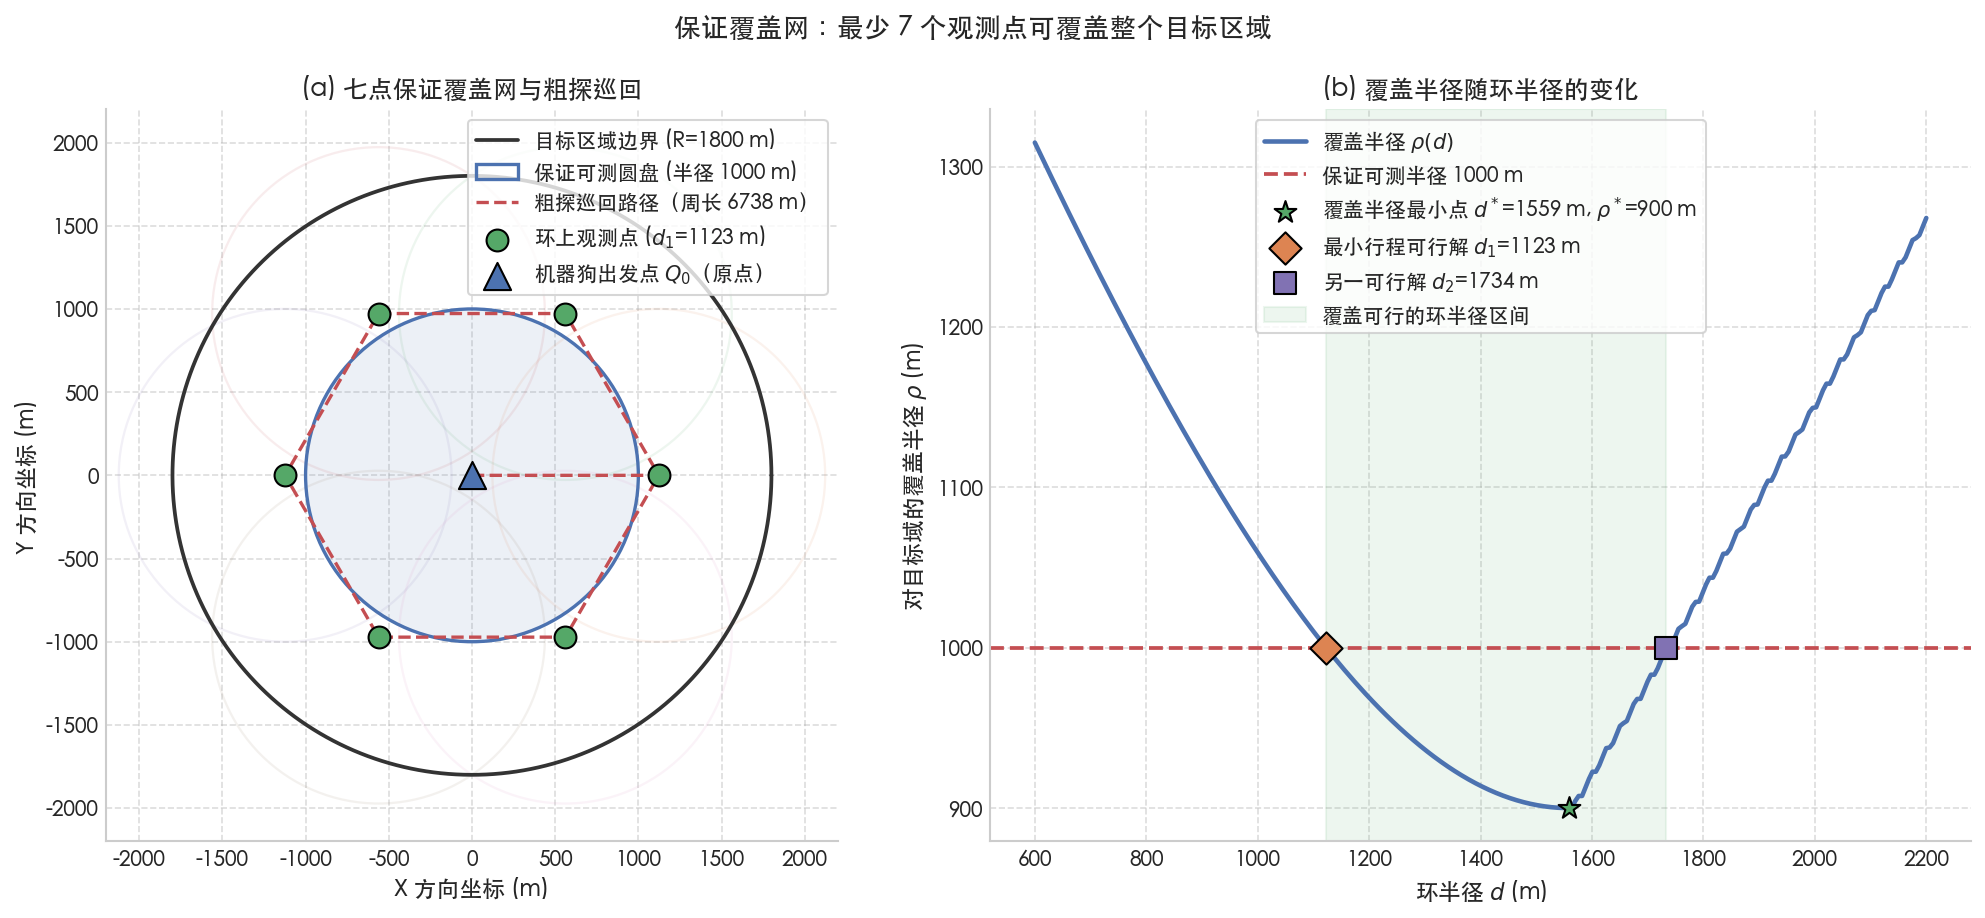
\includegraphics[width=0.8\textwidth]{问题三/figures/七点保证覆盖网示意图.png}
  \caption{七点保证覆盖网与覆盖半径随环半径的变化}
  \label{fig:r3-1}
\end{figure}

图 \ref{fig:r3-1}(a) 显示七个半径 $1000$ 米的圆盘恰好覆盖整个目标圆域；稠密采样 $1.5\times10^6$ 点验证最大最近邻距离为 $1000.000002$ 米，覆盖率 $99.999867\%$。图 \ref{fig:r3-1}(b) 显示覆盖半径曲线在 $d^{*}=1558.85$ 米处触底 $900$ 米，与 $1000$ 米门槛相交于 $d_1$、$d_2$ 两点。

\begin{figure}[H]
  \centering
  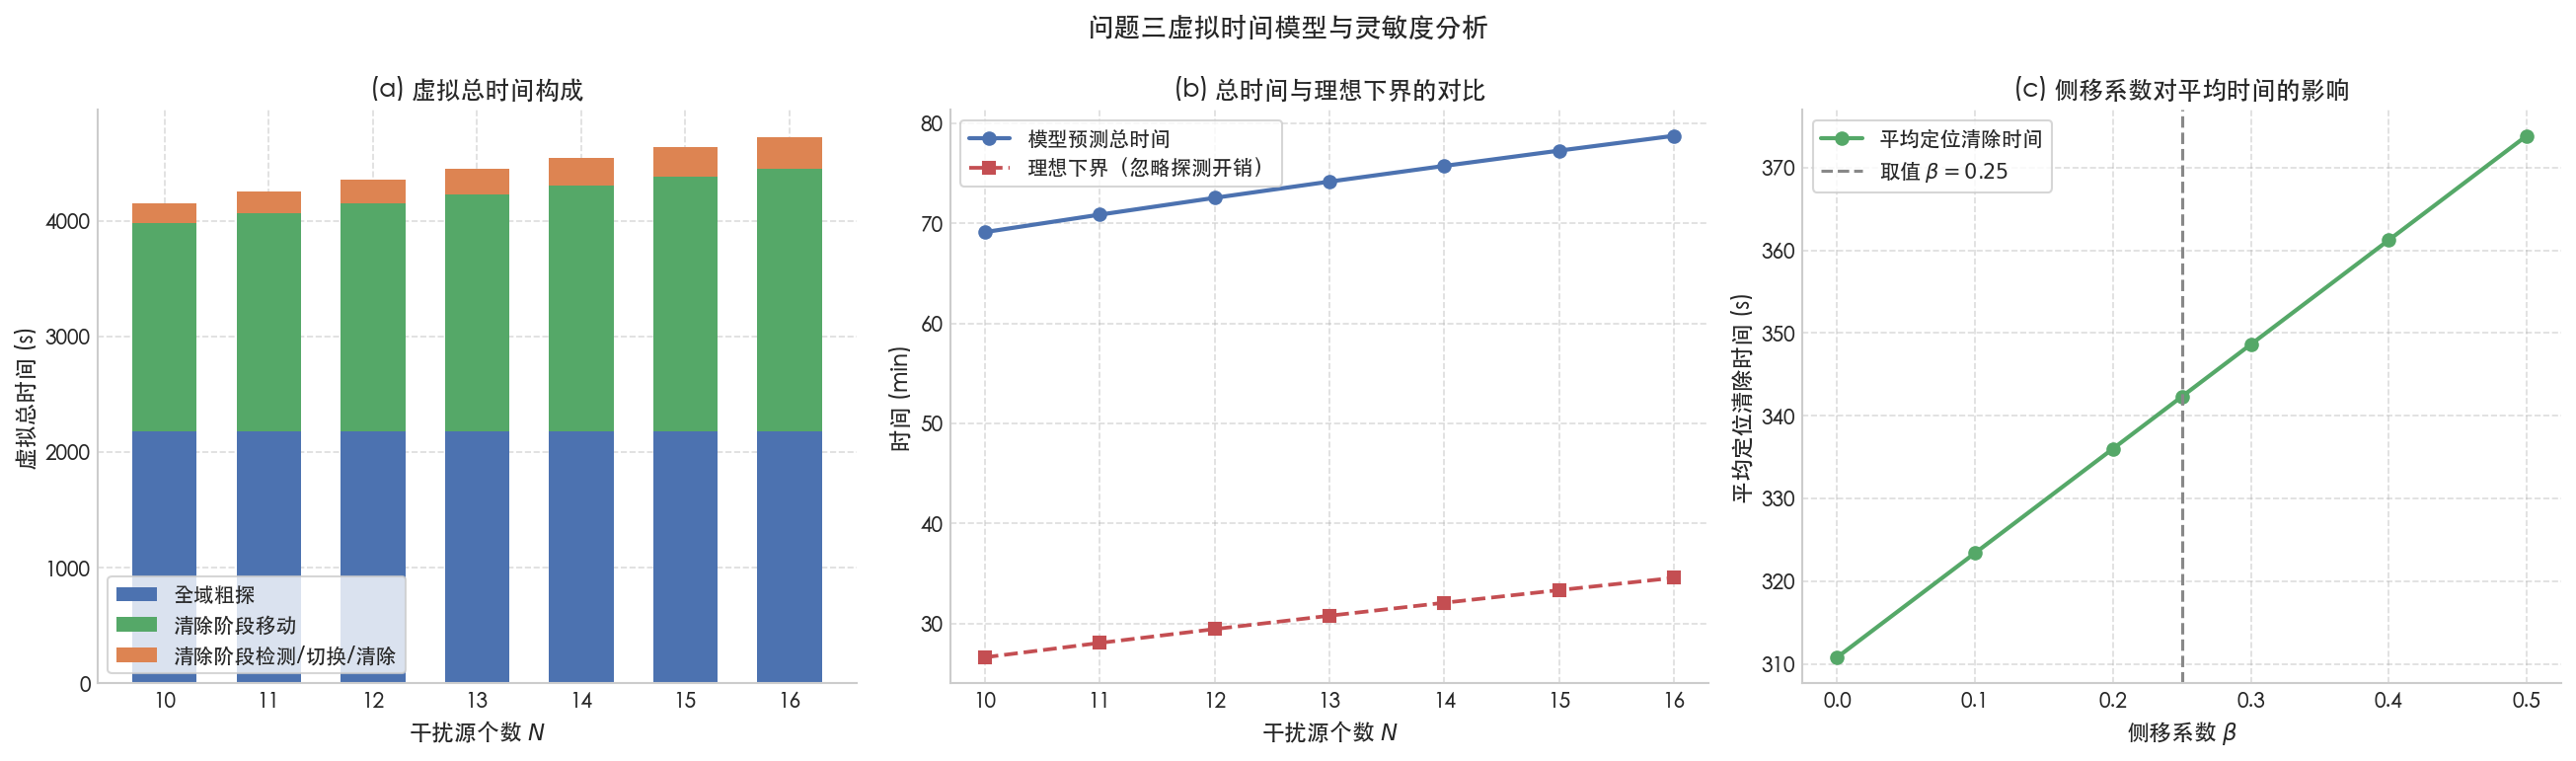
\includegraphics[width=0.8\textwidth]{问题三/figures/虚拟时间构成与灵敏度图.png}
  \caption{虚拟时间构成、与理想下界的对比及侧移系数灵敏度}
  \label{fig:r3-2}
\end{figure}

图 \ref{fig:r3-2}(b) 显示 $N=13$ 时模型总时间 $4450$ 秒与理想下界 $1847$ 秒的比值约为 $2.4$，差距全部来自保证全覆盖所必需的粗探开销。

% ============================================================
\section{问题四结果汇总}
% ============================================================

本问解决了"目标区域中同时存在全向与定向干扰源、定向方向未知"条件下的检测与清除问题。核心发现是：定向源的可检测域由圆盘收缩为半圆盘，使"无信号"退化为三义信息，问题三的保证覆盖网在定向场景下\textbf{必然漏测}，必须引入方位冗余。

本问给出两个可判定的定理。其一是背向不可测定理：若两个探测点对干扰源的视角差不少于 $180^\circ$ 且都在有效接收半径内，则二者不可能同时返回无信号；数值验证的 $4000$ 组构造中反例为 $0$ 组，单点无信号频率 $0.4960$ 与理论值 $0.5$ 吻合。其二是方位包围判据：
\begin{equation}
\text{零漏测}\iff \mathcal Q\cap\mathcal B(G,r_c)\ \text{的方位角最大间隔}<180^\circ
\iff G\in\operatorname{int}\operatorname{conv}\bigl(\mathcal Q\cap\mathcal B(G,r_c)\bigr).
\end{equation}

\begin{table}[H]
  \centering
  \caption{问题四关键结果}
  \label{tab:r4-key}
  \begin{tabularx}{\textwidth}{LC}
    \toprule
    指标 & 数值 \\
    \midrule
    七点覆盖网 全域最大方位间隔 & $360.00^\circ$（$\ge180^\circ$，存在漏测方向） \\
    七点覆盖网 平均漏测概率（定向方向随机） & $65.24\%$ \\
    七点覆盖网 必然漏测区（半径 $1200\sim1800$ m） & $100.00\%$ \\
    背向不可测定理 数值验证反例数 & $0$ / $4000$ \\
    单点探测无信号频率（对照） & $0.4960$（理论 $0.5$） \\
    \textbf{分级零漏测冗余网 最小规模} & $\mathbf{37}$ 点（环点数 $6/12/18$，半径 $1000/1300/1900$ m） \\
    冗余网 全域最大方位间隔 & $155.67^\circ$（$<180^\circ$，零漏测成立） \\
    静态方案粗探时间 & $8776.9$ s（问题三为 $2180.6$ s） \\
    \textbf{定向源时间惩罚系数} $\kappa_{\mathrm{static}}$ & $\mathbf{3.025}$ \\
    自适应方案总时间（$u=2$ 个未解频道） & $6561.8$ s（较静态方案节省 $25.2\%$） \\
    \bottomrule
  \end{tabularx}
\end{table}

表 \ref{tab:r4-key} 的核心结论是：要使综合场景下的漏测概率严格为零，静态冗余网需要 $37$ 个观测点、粗探时间 $8777$ 秒，是问题三的 $3.025$ 倍；而采用"七点粗探 $+$ 仅对未解频道沿加密环补测"的自适应策略，在未解频道数为 $2$ 时总时间为 $6562$ 秒，仍比静态方案节省 $25.2\%$，故推荐以自适应补测作为实际执行策略。

\begin{figure}[H]
  \centering
  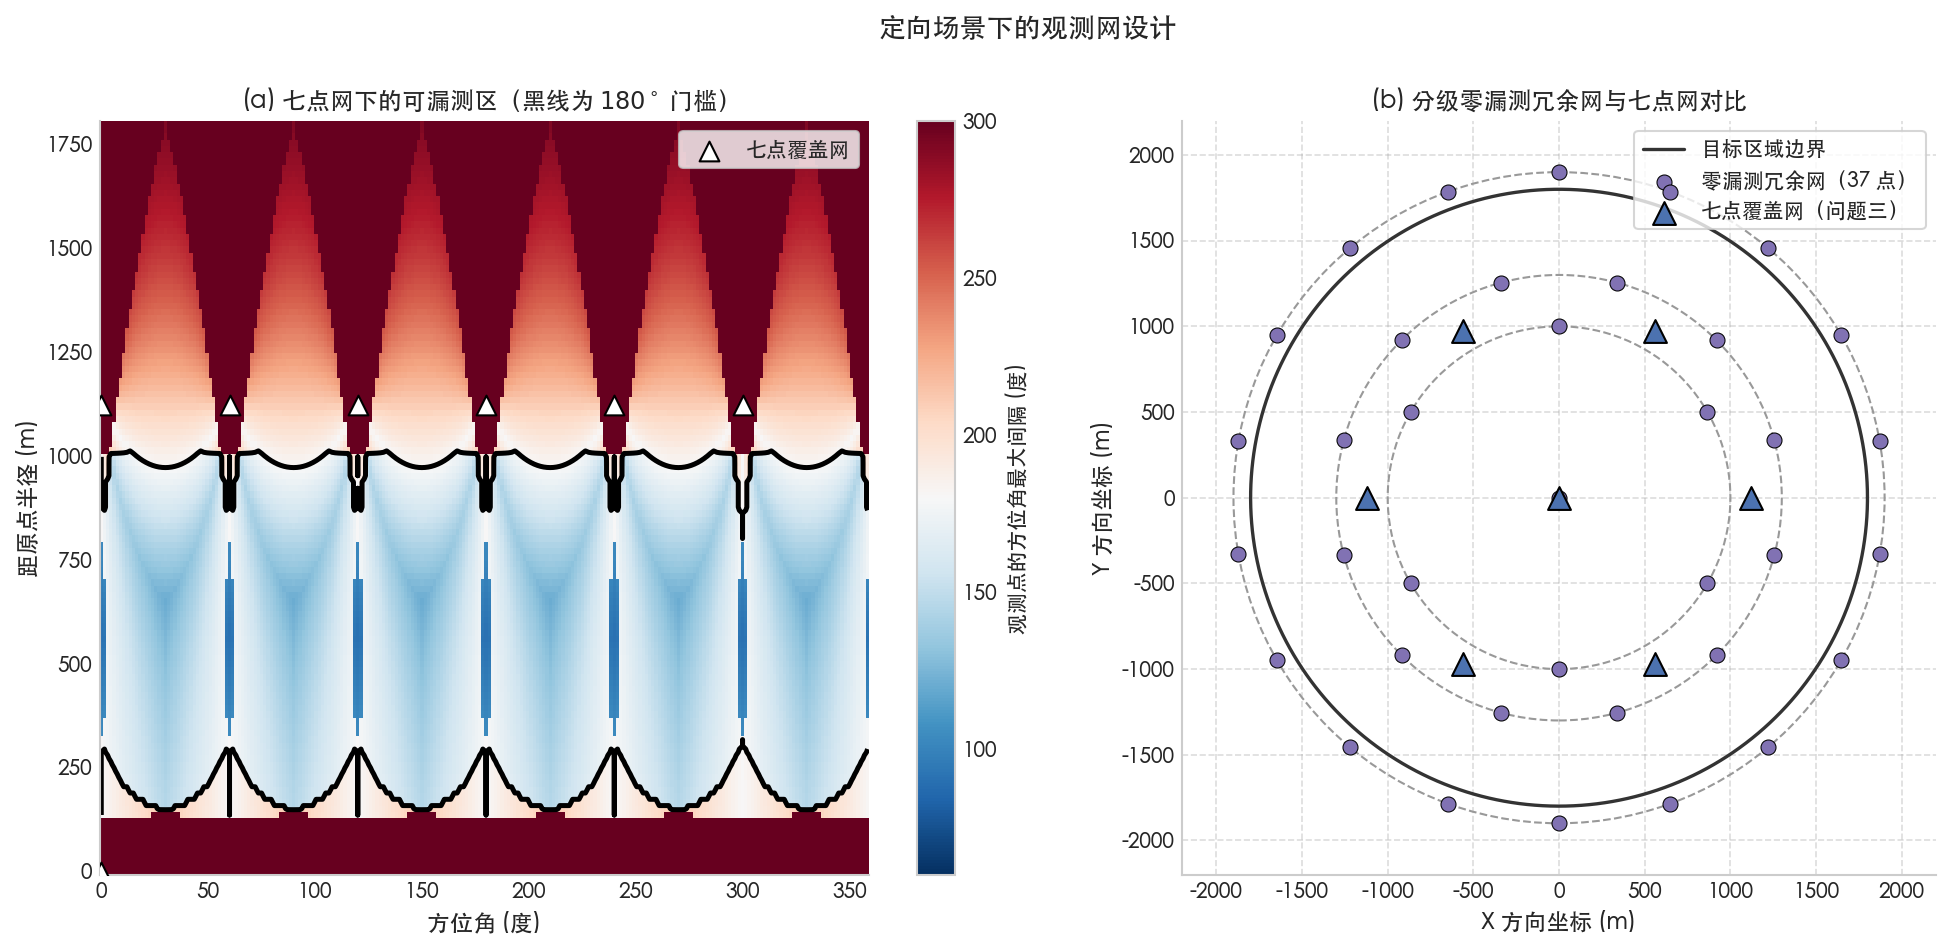
\includegraphics[width=0.8\textwidth]{问题四/figures/七点网可隐藏区与冗余网对比图.png}
  \caption{七点网下的可漏测区与分级零漏测冗余网}
  \label{fig:r4-1}
\end{figure}

图 \ref{fig:r4-1}(a) 以极坐标热力图呈现七点网的漏测风险：仅有一条狭窄的蓝色环带（约半径 $600$ 米）对任意定向方向都不会漏测，其余区域均存在漏测方向，半径 $1200$ 米以外则必然漏测。图 \ref{fig:r4-1}(b) 给出 $37$ 点分级冗余网与七点网的对比。

\begin{figure}[H]
  \centering
  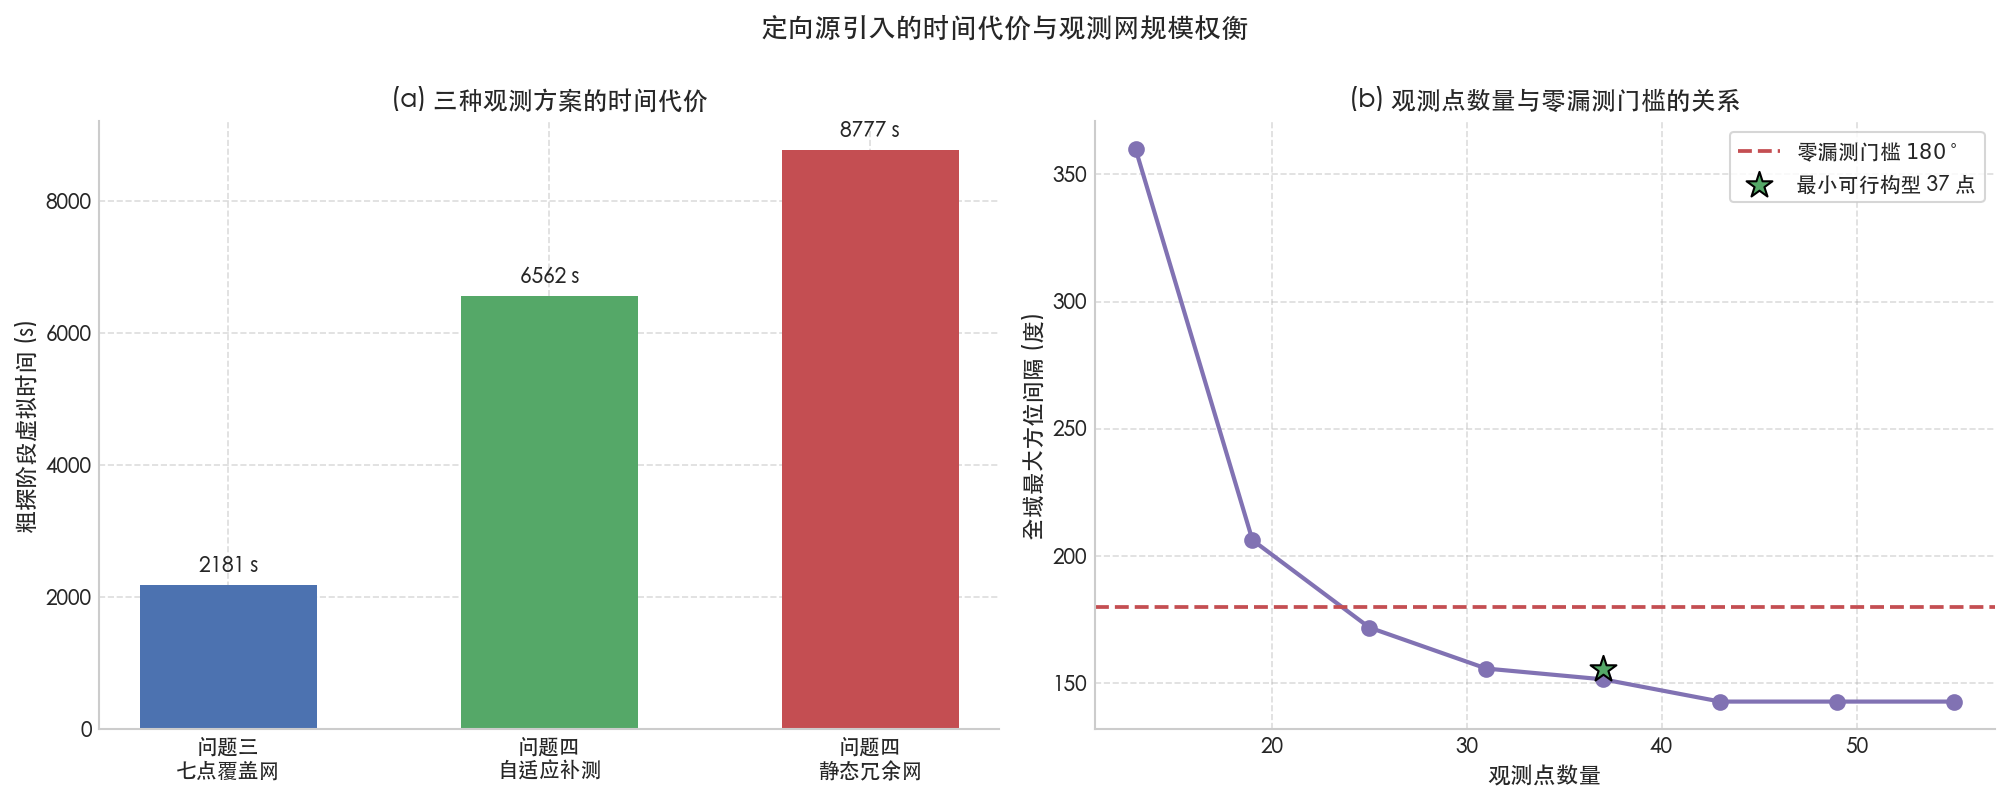
\includegraphics[width=0.8\textwidth]{问题四/figures/定向源时间惩罚与网规模权衡图.png}
  \caption{定向源引入的时间代价与观测网规模的权衡}
  \label{fig:r4-2}
\end{figure}

图 \ref{fig:r4-2}(b) 显示观测点数与最大方位间隔的关系曲线在 $37$ 点处穿过 $180^\circ$ 门槛，此后继续加密的边际收益迅速衰减。

% ============================================================
\section{综合结论}
% ============================================================

四个问题构成一条由几何到决策、由确定性到不完全观测的完整链条，本文的求解结果可以串联成如下故事。

问题一把"示向度"这一角度观测转化为可计算的位置集合。其结论是：单条示向度只给出张角 $2^\circ$ 的楔形，两条示向度的楔形求交给出凸四边形定位区域；该区域的直径可由旋转卡壳在 $O(h)$ 时间内精确求出，而以该直径为直径的圆\textbf{不能保证}覆盖该区域，覆盖成立的充要条件是两个非直径端点处的内角均不小于 $90^\circ$。在大规模随机构型中，覆盖率约为 $98.99\%$，失效仅出现在交会角接近 $90^\circ$ 的临界构型上，且失效的绝对幅度不超过 $1.17$ 米。

问题二把定位区域这一度量工具转化为布站决策。其结论是：对于已知距离 $r$ 的目标，垂直布站下的最优基线为 $b^*=\sqrt2r$，对应最优交会角 $54.74^\circ$ 与定位误差 $E_{\min}=3\delta r$；而在目标距离未知时，必须按可行域期望或最坏情形重新优化，所得最优布站为偏离示向度方向约 $20^\circ$、基线约 $1401$ 米，期望定位误差 $22.19$ 米；教科书中常被引用的垂直布站即使把基线放长到 $1510$ 米，期望误差仍高达 $55.73$ 米，是最优方案的 $2.5$ 倍。候选区域为以第一检测点为圆心、半径 $1230\sim1630$ 米、偏离示向度 $14^\circ\sim29^\circ$ 的两条对称圆弧带。

问题三把布站决策嵌入全域搜索任务。其结论是：要保证无论有效接收半径取何值 $D$ 内任何干扰源都可被测到，最少需要 $7$ 个观测点，其下界由 Kershner 定理给出，其最小行程构型为半径 $1122.96$ 米的六边形环加中心点；配合"侧移定距—迭代逼近—就地清除"的闭环，$N=13$ 时虚拟总时间的模型预测为 $4450$ 秒、平均定位清除时间 $342$ 秒，与理想下界 $1847$ 秒的比值约为 $2.4$，差距全部来自保证全覆盖所必需的探测开销。

问题四在问题三之上引入定向源，使"无信号"从弱信息退化为三义信息。其结论是：七点覆盖网在半径 $1200$ 米以外对定向源\textbf{必然漏测}，全域平均漏测概率 $65.24\%$；零漏测的充要条件是观测点在干扰源附近必须"包围"而非仅仅"覆盖"；在"中心加分级同心环"构型族内，满足零漏测的最小规模为 $37$ 点，代价是粗探时间增至 $8776.9$ 秒，相对问题三的惩罚系数为 $3.025$；而采用"七点粗探加自适应补测"的策略，在典型情形下可把总时间压至 $6562$ 秒，仍比静态方案节省 $25.2\%$。

从整体上看，本题的研究揭示了角度观测定位系统中一条贯穿始终的规律：\textbf{观测的几何结构比观测的数量更重要}。问题一说明定位区域的形状由交会角决定，问题二说明最优布站取决于交会角与距离的加权平衡，问题三说明探测点的布置必须兼顾覆盖与行程，问题四则进一步说明在存在方向性盲区时"覆盖"必须升级为"包围"。据此，对实际系统的建议有三条：其一，在测向设备选型上应优先提高角度精度，因为它同时改善定位精度、缩小逼近距离并降低时间代价，是全局杠杆最大的参数；其二，多站协同测向时应避免共线布站，并把基线长度与目标距离的估计值建立联动；其三，当被测目标可能存在方向性辐射时，观测网的密度必须按"方位包围"而非"距离覆盖"的标准设计，否则任何提高测向精度的努力都无法弥补漏测风险。

% ============================================================
\section{结果速查表}
% ============================================================

\begin{table}[H]
  \centering
  \caption{全部问题关键结果速查}
  \label{tab:quick}
  \begin{tabularx}{\textwidth}{CLC}
    \toprule
    问题 & 核心指标 & 数值 \\
    \midrule
    \multirow{5}{*}{问题一}
      & 直径圆覆盖率（纯交会四边形） & $98.99\%$ \\
      & 直径圆覆盖率（叠加圆域截断） & $96.28\%$ \\
      & 覆盖成立充要条件 & $\angle ABC\ge90^\circ$ 且 $\angle ADC\ge90^\circ$ \\
      & 定位区域直径 均值 / 中位数 & $402.53$ / $157.96$ m \\
      & 覆盖失败超出量 均值 / 最大值 & $0.4928$ / $1.1697$ m \\
    \midrule
    \multirow{5}{*}{问题二}
      & 垂直布站解析最优 & $b^*=\sqrt2r$，$\alpha^*=54.74^\circ$，$E_{\min}=3\delta r$ \\
      & 期望准则最优布站 & $b^*=1401.4$ m，$\varphi^*=20.03^\circ$ \\
      & 期望定位误差 & $22.19$ m \\
      & 垂直布站对照 & $b=1510$ m 时误差 $55.73$ m（$2.5$ 倍） \\
      & 候选区域 & $b\in[1230,1630]$ m，$\varphi\in[14^\circ,29^\circ]$ \\
    \midrule
    \multirow{5}{*}{问题三}
      & 最少保证观测点数 & $7$（Kershner 下界） \\
      & 最小行程环半径 $d_1$ & $1122.96$ m（覆盖半径 $1000$ m） \\
      & 覆盖网巡回路径 & $6737.7$ m \\
      & 粗探阶段时间 & $2180.5$ s（检测 $140$ 次，切换 $133$ 次） \\
      & 总时间 / 平均定位清除时间（$N=13$） & $4450.3$ s / $342.3$ s \\
      & 清除精度逼近阈值 & $r\le381.97$ m \\
      & 理想下界（$N=13$） & $1847.0$ s \\
    \midrule
    \multirow{6}{*}{问题四}
      & 七点网全域最大方位间隔 & $360.00^\circ$ \\
      & 七点网平均漏测概率 & $65.24\%$ \\
      & 零漏测判据 & 方位角最大间隔 $<180^\circ$ \\
      & 分级冗余网最小规模 & $37$ 点（环点数 $6/12/18$） \\
      & 冗余网最大方位间隔 & $155.67^\circ$ \\
      & 静态时间惩罚系数 $\kappa$ & $3.025$ \\
      & 自适应方案总时间（$u=2$） & $6561.8$ s（节省 $25.2\%$） \\
    \bottomrule
  \end{tabularx}
\end{table}

\end{document}
